% \documentclass{standalone}
% \usepackage{tikz}
% \usetikzlibrary{calc}
% \begin{document}

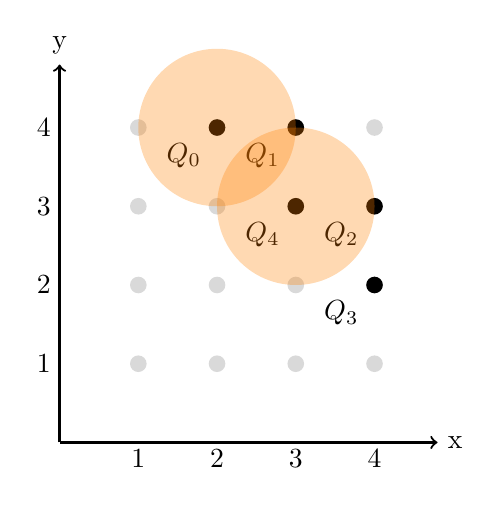
\begin{tikzpicture}
    % Helper styles for better readability
    \tikzstyle{unoccupied}=[fill=gray!30, circle, minimum size=6pt, inner sep=0pt]
    \tikzstyle{occupied}=[fill=black, circle, minimum size=6pt, inner sep=0pt]
    \tikzstyle{rydbery_circle}=[fill=orange, opacity=0.3]

    \begin{scope}[shift={(0,0)}]
        % Axes
        \draw[->, thick] (0, 0) -- (4.8, 0) node[right] {x};
        \draw[->, thick] (0, 0) -- (0, 4.8) node[above] {y};

        % x and y labels
        \foreach \x in {1, 2, 3, 4} {
            \node at (\x, -0.2) {\x};
        }
        \foreach \y in {1, 2, 3, 4} {
            \node at (-0.2, \y) {\y};
        }
    
        % Unoccupied nodes - dashed circles
        \foreach \x in {1, 2, 3, 4} {
            \foreach \y in {1, 2, 3, 4} {
                \node[unoccupied] at (\x, \y) {};
            }
        }
        
        % SLM occupied nodes (filled circles)
        \foreach [count=\i from 0] \x/\y in {2/4, 3/4, 4/3, 4/2, 3/3} {
            \node[occupied, label=below left:{$Q_{\i}$}] at (\x, \y) {};
        }
        
        % rydbery laser(circled filled circles), r = 1
        % \foreach \x/\y in {2/4, 3/4, 4/3, 4/2} {
        %     \fill[rydbery_circle] (\x, \y) circle (0.51);
        % }
        % r=2
        \foreach \x/\y in {2/4, 3/3} {
            \fill[rydbery_circle] (\x, \y) circle (1);
        }
        
        % Title
        % \node[below] at ($(2.5,-0.5)$) {b)};
    \end{scope}

\end{tikzpicture}

% \end{document}
